\Needspace{3in}
\begin{prob}

    Suppose Bellman-Ford with early stopping is run on the weighted graph below.
    The algorithm uses node $a$ as the source node.

    \begin{center} 
    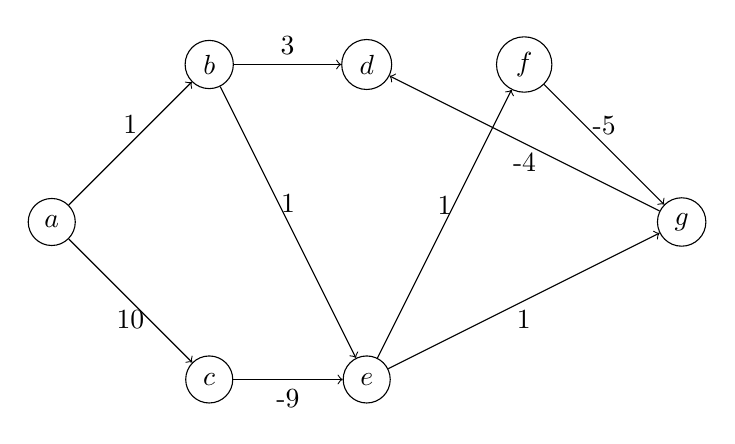
\begin{tikzpicture}
    {
        \tikzset{every node/.style = {shape=circle, draw, minimum size=17pt}}
        
        \node (a) at (0, 0) {$a$};
        \node (b) at (2, 2) {$b$};
        \node (c) at (2, -2) {$c$};
        \node (d) at (4, 2) {$d$};
        \node (e) at (4, -2) {$e$};
        \node (f) at (6, 2) {$f$};
        \node (g) at (8, 0) {$g$};
    }
        
        \draw (a) edge[->] node[above, midway] {1} (b);
        \draw (b) edge[->] node[above, midway] {1} (e);
        \draw (a) edge[->] node[below, midway] {10} (c);
        \draw (c) edge[->] node[below, midway] {-9} (e);
        \draw (e) edge[->] node[below, midway] {1} (g);
        \draw (f) edge[->] node[above, midway] {-5} (g);
        \draw (e) edge[->] node[above, midway] {1} (f);
        \draw (b) edge[->] node[above, midway] {3} (d);
        %\draw (d) edge[->] node[above, midway] {4} (f);
        \draw (g) edge[->] node[below, midway] {-4} (d);
        %\draw (a) edge[->] node[below, midway] {5} (d);
        

    \end{tikzpicture}
    \end{center}

    After the third iteration, name all nodes whose shortest path from $a$ are guaranteed to be estimated correctly.

    \begin{choices}
        \correctchoice $\{a,b,c,e,f\}$
        \choice $\{g,f\}$
        \choice $\{a,b,c,e,f,g\}$
        \choice $\{a,b,c,d,e,f\}$
        \choice $\{a,b,c,d\}$
    \end{choices}


\end{prob}
